%!TEX root = ../dokumentation.tex
\lstset{
	frame=single,
	keywordstyle=\color{blue},
	commentstyle=\color{green},
	numbers=left,
}

\chapter{Backend}

Im Backend des \textbf{Sudoku Helper}s findet die Datenverarbeitung statt. Das Backend stellt das Gegenstück zum Frontend dar. In diesem Kapitel wird die Programmarchitektur beschrieben und die wichtigsten Klassen des Backend vorgestellt. Hier werden auch alle umgesetzten Lösungstechniken aufgezählt und bereits einen kleinen Ausblick gegeben welche Strategien noch weiter implementiert werden könnten. Danach wird die Umsetzung der Strategien beispielhaft an zwei Strategien erklärt.


\section{Programmarchitektur}

Wie in Kapitel xx erwähnt ist die Programmarchitektur des \textbf{Sudoku Helper} in drei Komponenten unterteilt, um eine geringe Kopplung und eine hohe Skalierbarkeit zu erreichen. 

\subsection{Model}
Aufgrund einer geringen Menge an Daten wird keine Anbindung an eine Datenbank benötigt. Bei den Daten selbst handelt es sich nur um teilweise verschachtelte Listen, in in der \textit{SudokuBoard} Klasse gehalten werden. Für die Manipulation dieser Daten verfügt die Klasse \textit{SudokuBoard} über einige Funktionen, die dem Controller eine Verarbeitung und Nutzung der Daten ermöglicht.

Erweitert wird das Model durch die Implementierung der Lösungsstrategien und deren benötigten Komponenten, die das Anwenden der Strategien ermöglichen. Die Strategien werden über den Controller aufgerufen.

\subsection{View}
Die View ist für die Darstellung der Daten und für das Empfangen der Nutzereingaben zuständig. Sie dient dem Nutzer als Steuerung, welcher über die im folgenden Kapitel xx beschriebenen Funktionalitäten das Programm beeinflussen kann. Die Eingaben des Benutzers werden an den Controller weitergegeben, im Gegenzug liefert der Controller Informationen über die Daten, die dargestellt werden sollen. 

Die Struktur der Darstellung ist vorgegeben durch eine \ac{HTML} Datei, welche mittels einer \ac{CSS} Datei gestaltet und formatiert wird. In der \textit{client.js} Datei wird der Client initialisiert, die Verbindung zum Server aufgebaut und dient zur Kommunikation mit dem Controller. Die \textit{style.js} Datei dient zur DOM Manipulation sowie zur Änderung \ac{CSS} Eigenschaften, um die Repräsentation für den Nutzer anzupassen.

\subsection{Controller}
Die Datei \textit{app.py} repräsentiert den Controller, welcher als zentrale Schnittstelle dient. Er startet die Applikation durch das Starten des Flask Servers und definiert einige Endpunkte für den Client. Alle Aktionen werden durch den Benutzer ausgelöst, wobei die von der View empfangenen Befehle überprüft und entsprechend die Daten an das Model weitergeleitet werden. Im Spezialfall des Betätigens der Hilfefunktion wird die oben erwähnte Erweiterung des Models der Lösungsstrategien gebraucht. Die entsprechenden Daten zur Darstellung der Hilfefunktion werden der View übergeben, für den letzten Hilfsschritt, dem Anwenden der Strategie, werden die Informationen dem Model übergeben. Die Antwort des Models wird über den Controller der View übergeben und die Darstellung aktualisiert. 

\section{Serverseite}

Um die \textbf{Sudoku Helper} Anwendung zu realisieren müssen Server und Client miteinander kommunizieren. Im Falle von standardmäßigen \ac{HTTP} Requests die synchron verlaufen wird die Seite bei jedem Request neu geladen. Dieses Verhalten beeinflusst die \ac{UX} negativ, daher sollte von einer synchronen Übertragung abgesehen werden.

Eine naheliegende Alternative ist \ac{AJAX}, welches ein Konzept der asynchronen Datenübertragung darstellt und eine Datenübertragung ohne Neuladen der Seite ermöglichen sollte. Dennoch bieten WebSockets einige Vorteile gegenüber \ac{AJAX}. WebSockets werden benutzt um full-duplex Kommunikation zwischen Server und Client zu definieren. Sie konzentrieren sich auf echte Parallelität und Leistungsoptimierung. Wie in Abbildung \ref{fig:VergleichWeb} zu erkennen ist, lassen sich über WebSockets dauerhafte Verbindungen herstellen, wobei Overhead eingespart werden kann.   

\begin{figure}[htbp]
	\centering
	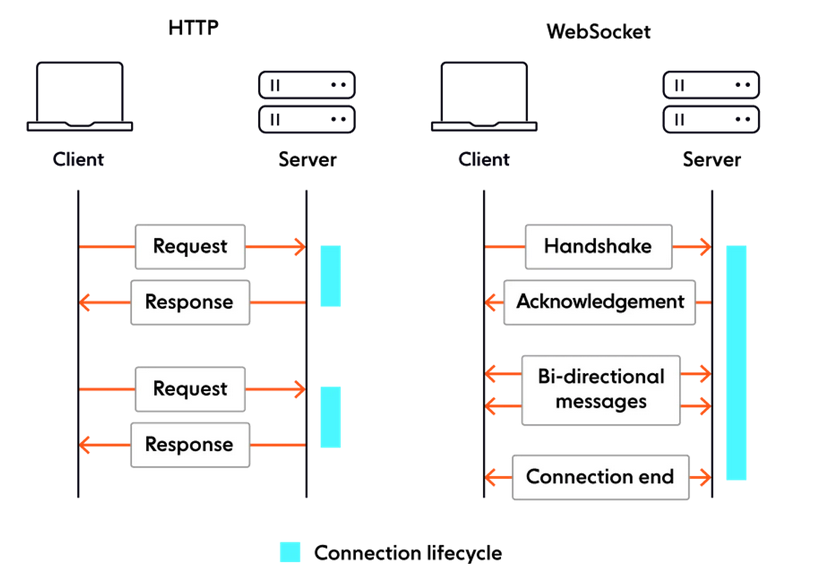
\includegraphics[width=0.5\textwidth]{images/Websocket.png}
	\caption{https://ably.com/blog/the-realtime-web-evolution-of-the-user-experience}
	\label{fig:VergleichWeb}
\end{figure}

In jedem Fall lassen sich mit einer WebSocket-Verbindung Bandbreite und CPU Zyklen einsparen. Für die Studienarbeit wird für die Kommunikation Serverseitig die Flask Erweiterung Flask-SocketIO verwendet.

\subsection{SocketIO}

Socket.IO ist eine Bibliothek, die eine bidirektionale und ereignisbasierte Kommunikation mit niedriger Latenz zwischen einem Client und einem Server ermöglicht. Die Hauptidee hinter Socket.IO ist, dass beliebige Ereignisse mit beliebigen Daten gesendet und empfangen werden können. Es baut auf dem WebSocket Protokoll auf und erweitert es mit Absicherungen wie die automatische Wiederverbindung von Clients und Verwendung von HTTP long-polling im falle von Kompatibilitätsproblemen.

Auf der Server-Seite erweitert die Socket-Instanz die EventEmitter-Klasse.

Auf der Client-Seite verwendet die Socket-Instanz den Ereignis-Emitter, der von der Komponenten-Emitter-Bibliothek bereitgestellt wird, die eine Teilmenge der EventEmitter-Methoden bereitstellt.

\section{SudokuBoard}

Ein wichtiger Part des Backend ist die Klasse \textit{SudokuBoard}. In dieser Klasse wird das Sudokuboard erstellt und eine Datenstruktur erschaffen in der die Informationen gespeichert werden. Aufgrund dieser Datenstruktur werden die Lösungsstrategien angewendet. In diesem Abschnitt wird die Datenstruktur erläutert und einige Funktionalitäten des SudokuBoard vorgestellt.

Die Zahlen und Kandidaten werden in unterschiedlichen Listen gespeichert. Das Board besteht aus einer zweidimensionalen List und die Kandidatennotation wurde mithilfe einer dreidimensionalen Liste umgesetzt. 

\subsection{Datenstruktur des Sudokuboards}
Die Zellenidentifikation ist in Abbildung \ref{fig:Sudokugitter} dargestellt. Der Inhalt der Zellen wird in einer Zweidimensionalen Liste gespeichert. Mit dem ersten Index wird eine Zeile ausgewählt und mit dem zweiten Index die Spalte. 

\begin{figure}[htbp]
	\centering
	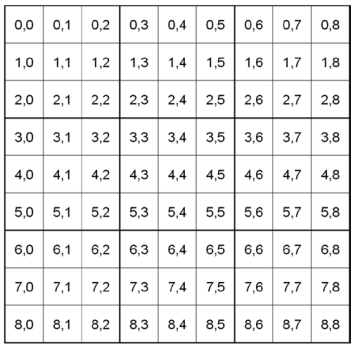
\includegraphics[width=0.3\textwidth]{images/board.png}
	\caption{Struktur des Sudokuboards und Zellenidentifikation \cite{zambon2015sudoku}}
	\label{fig:Sudokugitter}
\end{figure}

Wenn noch kein Board initialisiert wurde, dann wird die Datenstruktur erstellt und das gesamte Board mit Nullen befüllt. Diese Funktion ist in dem Codebeispiel \ref{lst:board} 

\begin{lstlisting}[caption={Initalisierung des Boards}, label={lst:board}]
	def init_board(self):
		self.board = []
		for i in range(SIZE):
			self.board.append([])
			for j in range(SIZE):
				self.board[i].append(0)
\end{lstlisting}

Die Kandidaten sind in einer dreidimensionalen Liste gespeichert. Mit den ersten beiden Indizes werden, genau wie auf dem Board die Zellen identifiziert. Die dritte Liste gibt Informationen über die Kandidaten in der entsprechenden Zelle. Die Liste hat eine Länge von neun, wobei jeder Eintrag entweder eine 0 oder eine 1 ist. Eine 1 bedeutet, dass ein Kandidat in einer Zelle ist. Der Nullte Index steht dabei für den Kandidaten eins.

\begin{lstlisting}[caption={Initalisierung der Kandidaten}, label={lst:candidates}]
	def init_candidates(self):
		for i in range(SIZE):
			self.candidates.append([])
			for j in range(SIZE):
				self.candidates[i].append([1] * SIZE)
\end{lstlisting}

Beim Initialisieren der Kandidaten, wie im Code \ref{lst:candidates} umgesetzt, werden zunächst alle Kandidaten gesetzt. Auf einem leeren Board könnte nämlich in jede Zelle jeder Wert, wenn noch keine Zahlen vorgegeben sind. Sobald dann Zahlen eingetragen werden, werden die Kandidatenwerte geupdated.

\subsection{Funktionalität}
Neben der Initialisierung des Boards und der Kandidaten, gehört das Prüfen der eindeutigen Lösbarkeit eines Sudoku Rätsel zu den wichtigsten Funktionalitäten der \textit{SudokuBoard} Klasse. Die Umsetzung dieser Funktionen wurde in dem Abschnitt \ref{eindeutigLösbar} und dem darauf folgendem bereits vorgestellt. Eine weiter wichtige Funktionalität dieser Klasse ist das updaten des Boards und der Kandidaten wenn Zahlen eingetragen sind. Auf diesen Datenstrukturen bauen alle Umsetzungen der Lösungstechniken auf. 

Des weiteren findet im \textit{SudokuBoard} die Umsetzung der Strategien statt. Dafür wurden die Funktionen \textit{remove\_candidates(self, cross\_outs)} und \textit{update\_numbers(self, number, cells)} implementiert. Hier wird eine weitere Unterscheidung zwischen Kandidaten und Zahlen getroffen. Kandidaten lassen sich nur entfernen, während es bei Zahlen sowohl das Löschen als auch das Hinzufügen möglich ist. Außerdem wird die Liste der Kandidaten nicht automatisch mit dem eintragen einer Zahl aktualisiert, sondern ausschließlich mit der letzten Hilfestellung.


\section{Technique Manager}

In der Datei \textit{technique\_manager.py} wird das Aufrufen der Techniken geregelt. 

Alle Lösungsstrategien sind als Klassenrepräsentation der umgesetzten Technik in einer Liste gespeichert. Weil die Techniken über eine abstrakte Klasse implementiert wurden, können alle Objekte unabhängig von der konkreten Implementierung im Technique Manager aufgerufen werden. Über diese Liste wird drüber iteriert und das Board und die Kandidaten übergeben. Danach wird die Methode \textit{execute\_technique()} für die Lösungstechnik ausgeführt. Der Returnwert dieser Methode ist True, wenn eine Technik anwendbar ist. In diesem Fall wird die Methode \textit{get\_result()} aufgerufen, welches ein Dictionary zurückgibt, indem alle benötigten Informationen für das Umsetzten der Hilfestellungen einer Lösungsstrategie enthalten sind.
Wenn eine Technik nicht erfolgreich ist dann wird mit der nächsten Lösungsstrategie aus der Liste weiter gemacht. 

Die Reihenfolge der Lösungstechniken ist von der Website \cite{martin} übernommen. Zuerst werden einfache Lösungsansätze ausprobiert und wenn diese nicht erfolgreich sind, werden immer komplexere Techniken angewendet. 

\begin{lstlisting}[language=Python, caption={Funktion um eine anwendbare Lösungstechnik zu finden}, label={lst:try}]
	def try_techniques(board, candidates):
		for tech in techniques:
			technique = tech(board, candidates)
			successful = technique.execute_technique()
			if successful:
				return technique.get_result()
		return False
\end{lstlisting}

\section{Abstrakte Klasse SolvingTechniques}

Wie im vorherigen Abschnitt des Technique Manager schon erwähnt gibt es eine Abstrakte Klasse Namens \textit{SolvingTechniques}, deren Funktionsweiße und Vorteile im weiteren Verlauf des Abschnittes erläutert wird. 

Mit einer Abstrakten Klasse kann ein gemeinsames Verhalten definiert werden. Dieses Verhalten wird von mehreren Unterklassen geerbt. Der Unterschied zwischen Klassen und abstrakten Klassen ist, dass von abstrakten Klassen keine Objekte erstellt werden können. Der Vorteil einer abstrakten Basisklasse ist die Nutzung mehrerer Unterklassen an einer gemeinsamen Programmierschnittstelle, in diesem Fall in dem \textit{TechniqueManager}. Zudem wird das gesamte Projekt durch das Einführen einer abstrakten Klasse übersichtlicher, da alle Unterklassen von dieser einen Klasse erben.

Diese abstrakte Klasse macht es dem Technique Manager möglich, alle Klassen der Lösungstechniken auf die selbe Weise zu instanziieren und zu verwenden. Mithilfe der abstrakten Klasse wird die Struktur der Lösungstechniken verallgemeinert, ohne dass jede Methode vollständig implementiert ist. 

Neben abstrakten Methoden sind noch weitere Funktionen in dieser Klasse implementiert die in mehreren Unterklassen verwendet werden können. Wenn eine Klasse also von einer abstrakten Klasse abgeleitet ist, so müssen alle abstrakten Methoden implementiert und überschrieben werden. 

\subsection{Abstrakte Methoden}
Die Verallgemeinerung der Lösungstechniken wird über abstrakte Methoden umgesetzt. Diese Methoden bieten die Standardfunktionalitäten der Basisklassen und müssen, wie schon erwähnt, implementiert werden. In Python können abstrakte Klassen erstellt werden, indem sie von dem ABC-Modul erben.

In der abstrakten Klasse \textit{SolvingTechniques} sind unter anderem drei verschiedene abstrakte Methoden deklariert. Diese brauchen in der abstrakten Klasse selbst keine Implementierung. Jede Klasse der Lösungstechniken braucht die Funktionen \textit{execute\_technique(self)}, \textit{configure\_highlighting(self)} und \textit{update\_explanation(self)}.

Mithilfe dieser drei abstrakten Methoden können alle Lösungstechniken übersichtlich implementiert werden. Nach Ausführen dieser Methoden wurde die Lösungstechnik auf das Sudoku angewendet. Dabei  wurden verschiedene Informationen in Variablen hinterlegt, die für den User mit der weiteren Benutzung der Hilfestellungen relevant sind.
Die Funktion der einzelnen Methoden wird in den folgenden Abschnitten erläutert. Im Zuge dessen werden auch die für das Frontend bereits erwähnten und wichtigen Variablen vorstellt, sowie der Grund des Erstellens.

\subsubsection{execute\_technique(self)}
In der Methode \textit{execute\_technique(self)} werden die Algorithmen für die spezifischen Techniken implementiert. Dabei wird zunächst nur überprüft, inwiefern eine Technik anwendbar ist. 

Wenn ein Algorithmus ein Muster für eine Technik erkennt und in der nächsten Methode Kandidaten zum rausstreichen gefunden werden, wird der Wert True zurückgegeben. Wenn keine passende Konstellation gefunden wird oder die Technik keine Auswirkung auf das aktuelle Board hat, dann wird ein False zurückgegeben.

\subsubsection{configure\_highlighting(self)}
Wenn ein Algorithmus eine Technik gefunden hat, dann wird in \textit{execute\_technique(self)} die abstrakte Methode 
\textit{configure\_highlighting(self)} aufgerufen. 

In dieser Methode werden die spezifischen Zellen und Kandidaten in denen die Technik gefunden wurde markiert. Dafür wurden in \textit{SolvingTechniques} Klassenvariablen angelegt. 
\begin{itemize}
	\item \textit{self.cross\_outs = []}
	\item \textit{self.highlights = []}
	\item \textit{self.primary\_cells = []}
	\item \textit{self.secondary\_cells = []}
\end{itemize}

Diese Variablen wurden schon im Frontend im Abschnitt \ref{Abstufung} erwähnt und deren Bedeutungen beschrieben. In den \textit{self.cross\_outs} werden Kandidaten bestimmter Zellen gespeichert, die laut Strategie entfernt werden können und in den \textit{self.highlights} werden Kandidaten aus bestimmten Zellen gespeichert, die eine besondere Bedeutung für die Strategie haben. Die \textit{self.primary\_cells} und \textit{self.secondary\_cells} enthalten nur Zellen, die für die Strategie relevant sind. Dabei sind die \textit{self.primary\_cells} tendenziell relevanter für Strategien und werden deutlicher hervorgehoben im Gegensatz zu den \textit{self.secondary\_cells}.

\subsubsection{update\_explanation(self)}
In \textit{update\_explanation(self)} wird eine Erklärung der Strategie gegeben. Diese Erläuterung wird in der Klassenvariable \textit{self.explanation} gespeichert. Bei der Erklärung wird darauf geachtet die Strategie an dem gefundenen Beispiel zu erläutern und den Grund zu nennen warum man diese Technik anwenden kann.

\subsection{Hilfsfunktionen}

In der abstrakten Klasse gibt es zusätzlich zu den abstrakten Methoden noch weitere Hilfsfunktionen. Diese Funktionen können in den Unterklassen aufgerufen werden, um die Implementierung zu erleichtern. Zu den wichtigsten Hilfsmethoden gehört \textit{get\_influential\_cells\_unit(cell, unit)}. Diese Methode gibt zu einer Zelle und einer Unit, alle Zellen die von der übergebenen Zelle in der spezifischen Unit gesehen werden, zurück. Für viele Strategien dient diese Funktion als Ausgangspunkt um bestimmte Muster auf dem Board zu erkennen.

Eine weitere sehr wichtige Methode ist \textit{get\_result(self)}. In dieser Methode werden die in \textit{configure\_highlighting(self)} gesammelten Informationen, der Technikname und die in der der Methode \textit{update\_explanation(self)} angepasste Beschreibung zurückgegeben. Die Informationen werden in einem Dictionary gespeichert und übergeben. 

\section{Lösungsstrategien}

In diesem Abschnitt wird ein Überblick über die implementierten Strategien gegeben. Die Lösungsstrategien sind auf der Website von Simon Martin \cite{martin} betitelt und beschrieben. Anhand diesen Beschreibungen wurden einige Lösungsstrategien implementiert. Zunächst wird ein Überblick über die umgesetzten Strategien gegeben, bevor ausblickend die Lösungsstrategien, die noch nicht implementiert wurden, aufgezählt werden. Es gibt noch weitere Strategien die auf der Website nicht beschrieben werden. Diese werden im Folgenden aber nicht weiter beachtet.

\subsection{Umgesetzte Lösungsstrategien}
Da in der Ausarbeitung nur exemplarisch auf einige wenige Lösungsstrategien eingegangen wird, sind in der Tabelle \ref{tab:implStrategien} alle implementierten Lösungsstrategien aufgezählt.
% Please add the following required packages to your document preamble:
% \usepackage{graphicx}
\begin{table}[H]
	\centering
	\resizebox{\textwidth}{!}{%
		\begin{tabular}{lllll}
			\cline{1-2} \cline{4-5}
			Technikname               & Technikname engl.          &  & Technikname               & Technikname engl.          \\ \cline{1-2} \cline{4-5} 
			Versteckter Single        & HiddenSingle               &  & Nackter Single            & Naked Single               \\
			Verstecktes Paar          & Hidden Pair                &  & Nacktes Paar              & Naked Pair                 \\
			Versteckter Dreier        & Hidden Triple              &  & Nackter Dreier            & Naked Triple               \\
			Versteckter Vierer        & Hidden Foursome            &  & Nackter Vierer            & Naked Foursome             \\
			Reihe-Block-Check         & Line-Block-Interaction     &  & Block-Reihe-Check         & Block-Line-Interaction     \\
			X-Wing                    & X-Wing                     &  & Steinbutt                 & Turbot                     \\
			Drittes Auge              & Third Eye                  &  & Wolkenkratzer             & Skyscraper                 \\
			Schwertfisch              & Swordfish                  &  & Drachen                   & Dragon                     \\
			Verbotenes Rechteck Typ 1 & Forbbiden Rectangle Type 1 &  & Verbotenes Rechteck Typ 2 & Forbbiden Rectangle Type 2 \\
			Verbotenes Rechteck Typ 3 & Forbidden Rectangle Type 3 &  & Verbotenes Rechteck Typ 4 & Forbidden Rectangle Type 4 \\
			XY-Wing                   & XY-Wing                    &  & XYZ-Wing                  & XYZ-Wing                   \\
			X-Kette                   & X-Chain                    &  & XY-Kette                  & XY-Chain                   \\
			Schwertfisch mit Flosse   & Swordfish with fin         &  &Doppelkette               & Double Chain                \\ \cline{1-2} \cline{4-5} 
		\end{tabular}%
	}
	\caption{Aufzählung aller implementierten Lösungsstrategien mit deutschem und englischem Bezeichner}
	\label{tab:implStrategien}
\end{table}

\subsection{Weitere Lösungsstrategien}
In der Studienarbeit wurden nicht alle auf der Website \cite{martin} vorgestellten Lösungstechniken umgesetzt. Weitere Strategien die noch implementiert werden könnten sind die folgenden:
\begin{itemize}
	\item Erweiterter \ac{BRC}
	\item W-Wing
	\item Geklonte Paare
	\item Leeres Rechteck
	\item Forcing Chain
\end{itemize}

Der Erweiterte \ac{BRC} wurde nicht umgesetzt, weil es eine Kombination aus dem \ac{BRC} und einem Versteckten Single ist. Außerdem wurde die Forcing Chain nicht implementiert, weil sie von der XY-Kette beinhaltet wird.

\section{Beispielhafte Umsetzung von Strategien}
Die Lösungsstrategien können zwei unterschiedliche Wirkungen auf ein Sudoku Rätsel haben. Entweder es ist möglich eine Zahl einzufügen oder es können Kandidaten aus verschiedenen Gründen eliminiert werden. Diese beiden Wirkungen werden im Backend unterschiedlich behandelt. In den nächsten zwei Unterkapiteln wird die Funktionsweise und die Unterschiede beider Varianten anhand zweier Beispiele erklärt. 

Für beide Umsetzungen wird die Abstrakte Klasse \textit{SolvingTechniques} genutzt.

\subsection{Zahl einfügen}

Der Fall, dass aufgrund einer Lösungstechnik direkt eine Zahl in das Sudokugitter eingetragen werden kann, gibt es in den umgesetzten Techniken nur in drei Fällen. Die anderen Techniken führen lediglich zu dem Rausstreichen von Kandidaten, woraufhin eventuell eine Zahl eingefügt werden kann.
\begin{itemize}
	\item Versteckter Single
	\item Nackter Single
	\item Drittes Auge
\end{itemize}

Für das Beispiel wird die Strategie des Nacktem Singles erklärt. Bei einem Nacktem Single steht in einer Zelle nur noch ein einziger Kandidat. Dieser Wert kann damit in die Zelle eingetragen werden.

Sobald auf dem Numpad der \textit{Help} Button das erste mal gedrückt wird, wird die Funktion \textit{try\_techniques()} im \textit{TechniqueManager} ausgeführt. 
\begin{lstlisting}[caption={Serverseitig help}, label={lst:helper}]
@socketio.on('help')
def help():
	global help_step
	global technique_result
	...
	if help_step == 0:
		sudoku.update_candidates()
		technique_result = technique_manager.try_techniques(sudoku.board, sudoku.candidates)
		if not technique_result:
			print("No suitable technique found!")
			return
		emit('help0', {'name': technique_result['name'], 'primaryCells': technique_result['primary_cells'], 'secondaryCells': technique_result['secondary_cells']})
\end{lstlisting}

Zunächst wird die Liste der Techniken im \textit{TechniqueManager} durch iteriert. An der Stelle des Versteckten Singles wird von der abstrakten Methode \textit{execute\_technique(self)} True zurückgegeben. Die Funktion ist in dem Codebeispiel \ref{lst:NakedSingle} abgebildet. Der Algorithmus loopt über alle Zellen auf dem Board. Wenn in einer Zelle eine Zahl steht die nicht Null ist, dass heißt beriets eine Zahl eingetragen ist, dann wird diese übersprungen. Da ein Kandidat über eine 1 dargestellt wird, lässt sich über die Summe aller Kandidaten in dieser Zelle auf die Anzahl an Kandidaten zurückschließen. Durch die Bedingung in Zeile 6 werden weiterhin alle Zellen übersprungen in denen mehr als ein Kandidat steht. Wenn eine Zelle nur einen Kandidaten hat, dann wird in dieser Zelle ein Nackter Single erkannt und zu den \textit{self.primary\_cells} hinzugefügt. Als nächstes wird die abstrakte Funktion \textit{configure\_highlighting(self)} aufgerufen. 

\begin{lstlisting}[caption={Nackter Single}, label={lst:NakedSingle}]
	def execute_technique(self):
		for i in range(9):
			for j in range(9):
				if self.board[i][j] != 0:
					continue
				if sum(self.candidates[i][j]) != 1:
					continue
				self.primary_cells = [(i, j)]
				self.configure_highlighting()
				return True
		return False
\end{lstlisting}

Auf das erfolgreiche Erkennen einer Strategie wird die Hilfsmethode \textit{get\_result()} für das Objekt des Versteckten Singles aufgerufen. Diese Ergebnisse sind nun in der globalen Variable \textit{technique\_result} gespeichert. Für jede weitere Hilfestellung wird der \textit{help\_step} um inkrementiert. Über \textit{emit} kann ein Event, dessen Callback in diesem Fall bei 'help0' definiert ist, ausgeführt werden. Die 'help0' Funktion wurde im Frontend in dem Abschnitt \ref{Abstufung} vorgestellt. Mit dem \textit{emit} werden zudem die gebrauchten Informationen übergeben.

Die nächsten beiden Hilfestellungen funktionieren auf die selbe Art und Weise. Erst bei der letzten Hilfestellung, dem Anwenden der Strategie, wird die einzig nötige Unterscheidung getroffen. Wie in dem Codebeispiel \ref{lst:helper1} gezeigt, wird der Name der Technik abgefragt. Wenn es eine der drei Techniken ist, bei denen eine Zahl auf dem Gitter eingefügt wird, dann wird die Funktion \textit{new\_number()} aufgerufen. Dieser Funktion wird die Zelle und die Zahl übergeben. Diese Werte bekommt man aus den \textit{self.highlights}.

\begin{lstlisting}[caption={Serverseitige Unterscheidung der zwei Arten von Techniken}, label={lst:helper1}]
	elif help_step == 3:
		if technique_result['name'] in ['Naked Single', 'Hidden Single', 'Third Eye']:
			data = {'number': technique_result['highlights'][0]['value'], 'checkedCells': [technique_result['highlights'][0]['cell']]}
			emit('help3')
			new_numbers(data)
			help_step -= 1
		else:
			sudoku.remove_candidates(technique_result['cross_outs'])
			candidates()
			emit('help3')
\end{lstlisting}

%Da die serverseitige Implementierung hier aufgeteilt vorgestellt wird, ist die ganze Funktion nochmals im Anhang \ref{lst:helpers} zu sehen.

\subsection{Kandidaten eliminieren}

Die Funktionsweise von Strategien die Kandidaten eliminieren ist ähnlich wie gerade beschrieben. Der einzige Unterschied ist, dass anstatt \textit{new\_number()} die Funktion \textit{remove\_candidate()} aufgerufen wird. Der optische Output wird wieder über \textit{emit}s organisiert. Aus diesem Grund wird für die Lösungsstrategie Versteckter Vierer nur die \textit{execute\_technique(self)} erläutert. 

Bei einem Verstecktem Vierer wird darauf überprüft ob vier Kandidaten in genau vier unterschiedlichen Zellen einer Unit vorkommen. Wenn dies der Fall müssen die vier Kandidaten in den vier Zellen stehen, daher können aus diesen vier Zellen alle anderen Kandidaten entfernt werden.

Da diese Technik in jeder Unit vorkommen kann, wird zu Beginn über jede Art von Unit geloopt, da es jede Unit neun mal gibt müssen für jede Art von Unit neun Iterationen durchgeführt werden. Für jede Unit werden alle vorkommenden Kandidaten aufgelistet.

Aus der Liste mit den Kandidaten werden alle Kombinationen ohne Wiederholungen gebildet. In den Zellen einer Unit wird mittels einer List comprehension überprüft in welchen Zellen die Kandidaten der Kombination vorkommen. Diese werden zur Liste \textit{matches} hinzugefügt. Nachdem über alle Zellen iteriert wurde, wird die Länge der Liste auf vier überprüft. Dieser Teil der Strategie ist in dem Codebeispiel \ref{lst:hiddenFoursome2} implementiert. 

Der vorletzte Schritt ist das Festlegen der Markierungen. Dafür wird hier wie zuvor beschrieben die abstrakte Methode \textit{configure\_highlighting(self)} aufgerufen. Als letztes wird überprüft ob Kandidaten herausgestrichen werden können. Wenn die Liste der \textit{self.cross\_outs} größer als Null ist, dann wird der Wert True zurückgegeben. Wenn keine Kandidaten herausgestrichen werden können, dann wird mit der nächsten Unit auf die zuvor beschriebene Art und Weise verfahren.

\begin{lstlisting}[caption={Erster Teil der Strategie Versteckter Vierer}, label={lst:hiddenFoursome2}]
	combos = set(combinations(occurring_candidates, 4))
	for self.combo in combos:
		matches = []
		for cell in self.unit_cells:
			...
			candidates_num = SolvingTechniques.format_candidates(self.candidates[x][y])
			if any(c in self.combo for c in candidates_num):
				matches.append(cell)
		if len(matches) == 4:
			self.primary_cells = matches
			self.configure_highlighting()
			if len(self.cross_outs) != 0:
				return True
\end{lstlisting}

Wenn in keiner Unit ein versteckter Vierer entdeckt wird von dem Algorithmus, dann gibt die Funktion False zurück und das Programm macht mit der nächsten Lösungsmethode weiter.